To find an appropriate balance between computational (CPU) time and accuracy of the solution, we perform a so-called mesh convergence.
We compare the same simulation using an increasingly finer mesh, which can be observed in figure \ref{fig:mesh-convergence}.

The results are tabulated in Table \ref{tb:mesh-convergence}.
Most importantly, the total displacements for the coarsest and finest mesh are within 10\% of each other, but the increase in computational time is considerable.
Bear in mind these are relative numbers, so towards the final simulations of this project we are looking at multiple hours per simulation if we were to use the finest mesh.
It is perfectly reasonable to use the larger (coarser) mesh sizes given the scope of this study, but we were happy with computational times for \SI{2.5}{mm}.

\begin{table}[h] \centering
    \begin{tabular}{ccc}
        \textbf{Mesh size [\si{\milli\metre}]} & \textbf{Total CPU time [\si{\second}]} & \textbf{Displacement, magnitude [\si{\nano\metre}]}\\ \hline
          10 & 14  & 68\\
           5 & 17  & 67\\
         2.5 & 47  & 63\\
        1.25 & 303 & 62
    \end{tabular}
    \caption[Mesh convergence]{Mesh convergence. Given the massive increase in computational }
    \label{tb:mesh-convergence}
\end{table}


\begin{figure} \centering
\begin{subfigure}{0.4\textwidth}
    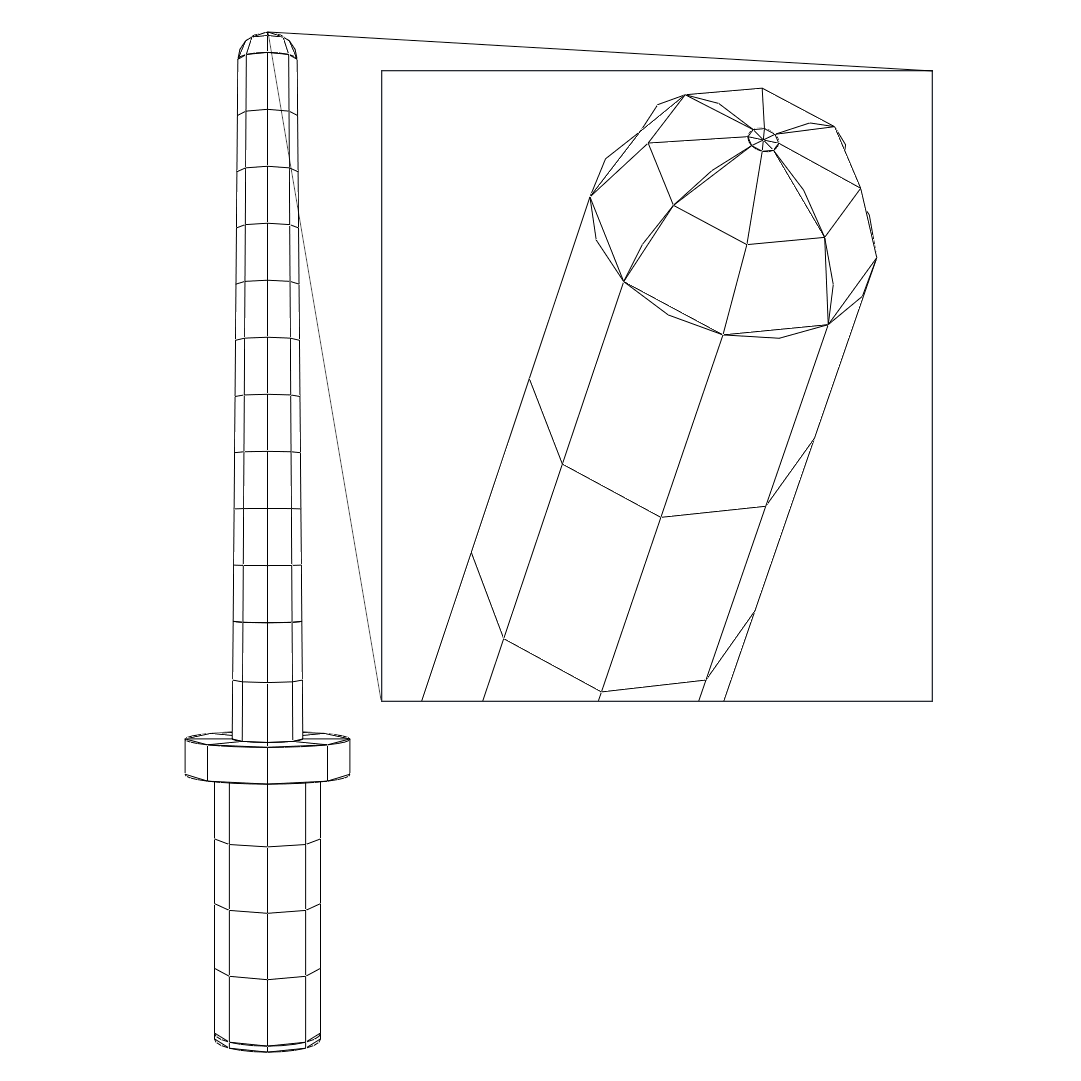
\includegraphics[width=\textwidth]{figures/0.01-finished.png}
    \caption{\SI{10}{\milli\metre}}
\end{subfigure}
\begin{subfigure}{0.4\textwidth}
    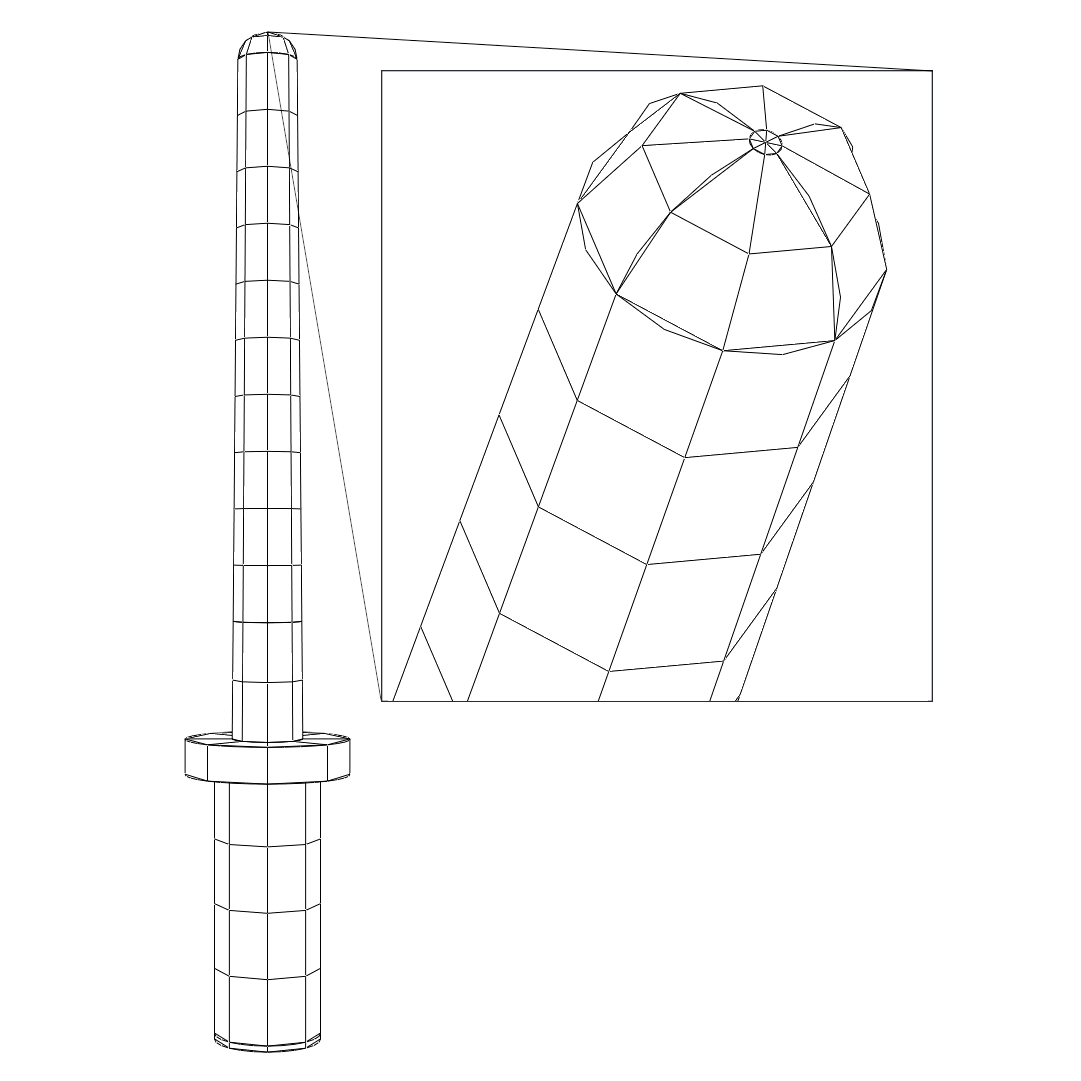
\includegraphics[width=\textwidth]{figures/0.005-finished.png}
    \caption{\SI{5}{\milli\metre}}
\end{subfigure}
\begin{subfigure}{0.4\textwidth}
    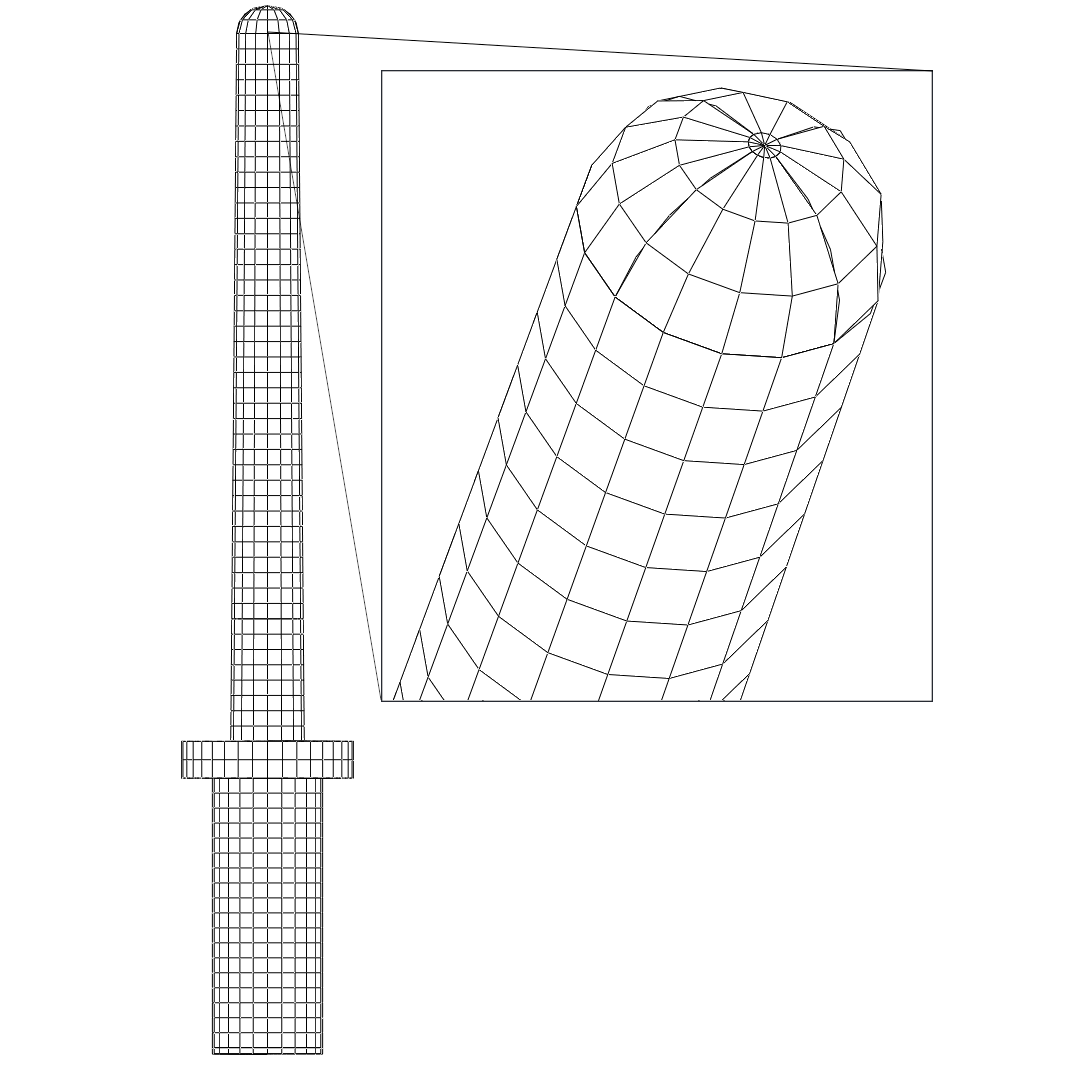
\includegraphics[width=\textwidth]{figures/0.0025-finished.png}
    \caption{\SI{2.5}{\milli\metre}}
\end{subfigure}
\begin{subfigure}{0.4\textwidth}
    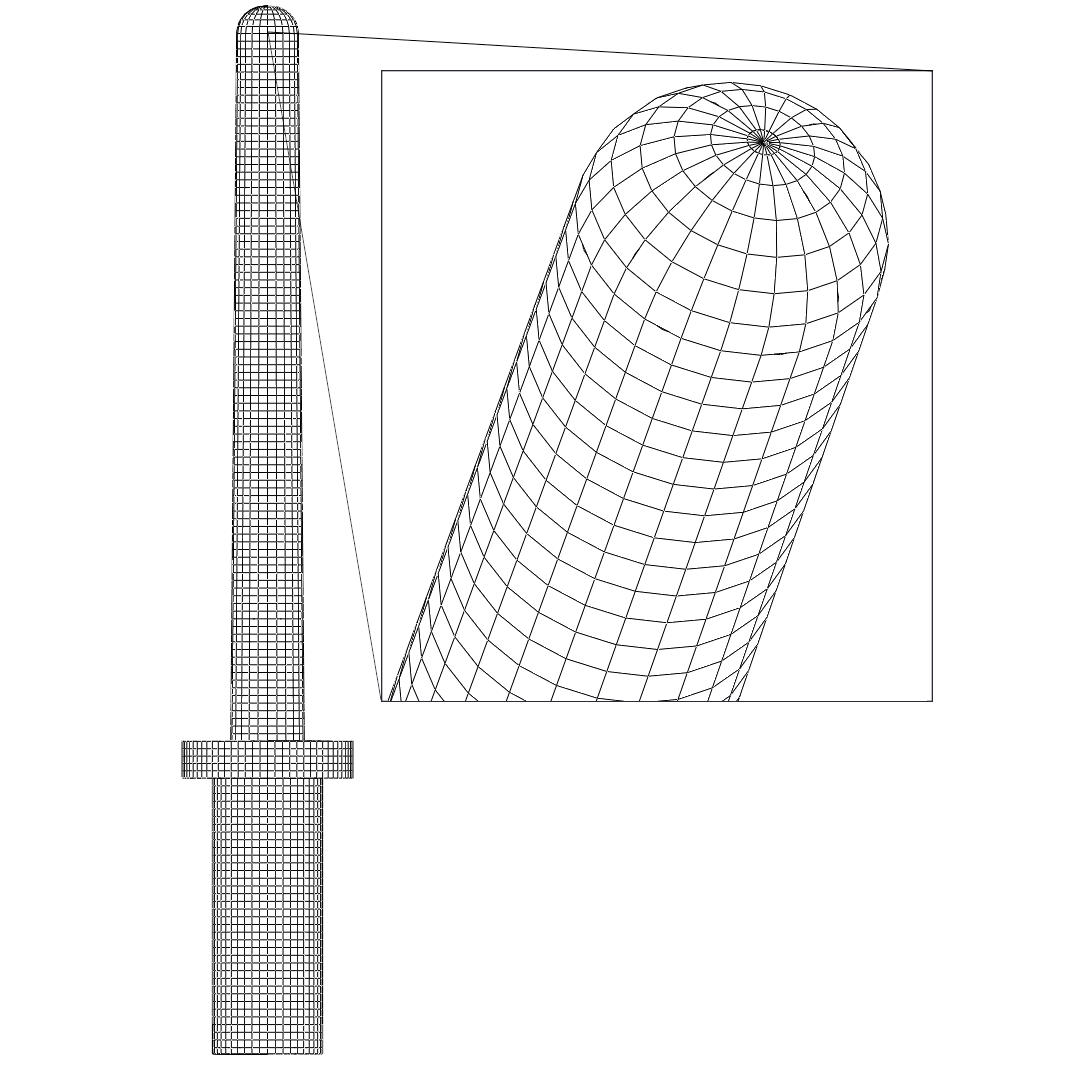
\includegraphics[width=\textwidth]{figures/0.00125-finished.png}
    \caption{\SI{1.25}{\milli\metre}}
\end{subfigure}
\caption{Mesh refinement from 10mm to 1.25mm}
\label{fig:mesh-convergence}
\end{figure}